\documentclass[12pt]{article}
\usepackage[utf8]{inputenc}
\usepackage{amsmath}
\usepackage{graphicx}
\usepackage[ruled, vlined]{algorithm2e}
\usepackage{algpseudocode}
\usepackage{caption}
\usepackage{subcaption}

\graphicspath{ {./images/} }

\title{On Synchronization Algorithms for the Optimization of Resources in Agriculture}
\author{Leonardo D. Garcia}
\date{\today}

\begin{document}

\maketitle

\begin{abstract}
This report examines a systems-based approach on the synchronization and optimization of resources in the agriculture sector. By providing an algorithmic aspect inspired by the dining philosophers problem from operating systems theory and multiplexing techniques from computer networks theory, it is possible to generate a concurrent program that will simulate the system dynamics of the plant models considering the sharing of limited resources such as water.
\end{abstract}

\small
\textbf{\textit{Keywords:}} multithreading, irrigation, algorithm, resources, multiplexing.

\section{Objectives}
The objectives of this paper focus on the capability of the present individual to formalize a contemporary viewpoint into the techniques that can be used in control engineering for the regulation and stability of dynamical systems.

Operating systems are the software pillars that holds together the organized aspects of the computer architecture. Although a computer by itself can work properly, the operating system controls and coordinates the management of physical resources inside the machine to provide the swiftest and best regulated of computing procedures.

Given the accelerated abilities of the processors, it has been proposed that one can employ the very same algorithms that the OS utilizes for their handling of shared data and memory locations in a similar way that generates an analogy to the inputs to withhold the stability of a plant—an irrigation area that must share its water with other adjacent sectors.

In essence, the purpose of this experiment is in the adaptation of a concurrent, synchronization algorithm from operating systems theory into a simple yet elegant solution that can be used for the reservation of input energy. At the same time, a similarly powerful alternative is demonstrated from the great utilities of computer network protocols.

\section{Theoretical Framework}

\subsection{Irrigation Areas}

An irrigation area is a finite-sized polygonal space where crops are grown throughout the year’s seasons. Like other real functional systems, they can be modeled mathematically as a linear-time invariant (LTI) system. A disadvantage in trying to do so lies on the fact that real systems usually present nonlinearities which complicate their analysis.

An alternative to preserve the advantages and strengths of an LTI system is by linearizing the plant on different operating points. As a result, a piecewise model of the plant is generated.

For this LTI models, a state-space approach is taken instead of a transfer function model to consider the controllability and observability of the plant for a MIMO model \cite{ogata}. The state equations for these cases are presented in Equations \ref{eqn:1} \& \ref{eqn:2}.

\begin{equation}
\label{eqn:1}
\mathbf{\dot{x}}(t) = \mathbf{A x}(t) + \mathbf{B u}(t)
\end{equation}
\begin{equation}
\label{eqn:2}
\mathbf{y}(t) = \mathbf{C x}(t) + \mathbf{D u}(t)
\end{equation}

$\mathbf{A}$ is the state matrix, $\mathbf{B}$ is the input matrix, $\mathbf{C}$ is the output matrix, and $\mathbf{D}$ is the transmission matrix. To avoid any major complication with the study of the irrigation areas, second-order models were identified from each of four distinct areas in previous studies from Dr. Camilo Lozoya.

These models depend thus on two state variables and two input variables. The state variables are the soil moisture $\theta(t)$ and the rate of change of the moisture with respect to time $\dot{\theta}(t)$. The input variables are from the other hand the irrigation level $ir(t)$ and the evapotranspiration (ETO) of the soil. The ETO is modified by a proportional parameter called $K_c$, which is denominated the crop constant and is a dimensional constant to regulate every area \cite{camilo2}. These change from area to area.

In the end, the vector expressions for these variables are displayed in Equations \ref{eqn:3} \& \ref{eqn:4}.

\begin{equation}
\label{eqn:3}
\mathbf{x}(t) = 
\begin{bmatrix}
\theta(t) & \dot{\theta}(t)
\end{bmatrix}
^T
\end{equation}
\begin{equation}
\label{eqn:4}
\mathbf{u}(t) = 
\begin{bmatrix}
ir(t) & K_c ETO(t)
\end{bmatrix}
^T
\end{equation}

The actual state equations must be separated according to three levels. The denominated previous investigations from Dr. Lozoya categorize the advancements of water consumption unto two thresholds \cite{camilo1}. The first threshold separates what is considered the gravitational water, which is the excess water that remains after an irrigation cycle. It can be found at the top of the moisture level diagram.

The next phase is the stable region, which is the most preferrable because it keeps in place the safety of the plant. No hazardous risks relating to water shortage occur at this point. There is a middle bias line that represents the most optimal operating point for the area. This specific offset depends on the irrigation area and most of the times can only be estimated experimentally.

Hydric stress then becomes an urgent problem once the plant leaves the stable region. It is at this point where the lack of water becomes significant to the vegetation and therefore can spawn visible damage sooner or later pertaining to the drought of the crop region. Fig. \ref{fig:dyn} depicts a crude diagram of these operating zones for a sample model.

\begin{figure}[ht]
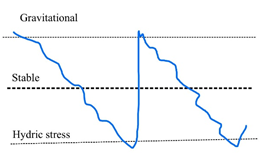
\includegraphics{dynamics}
\centering
\caption{Levels of soil moisture for the plant.}
\label{fig:dyn}
\end{figure}

In total, three state matrices and three input matrices were formed depending on the level of water consumption present \cite{camilo3}. These are presented as Equations \ref{eqn:5} to \ref{eqn:10} here below.

\begin{equation}
\label{eqn:5}
\mathbf{A}_{above}(t) = 
\begin{bmatrix}
0.98501 & 0.00001 \\
0.00001 & 0.98501
\end{bmatrix}
\end{equation}

\begin{equation}
\label{eqn:6}
\mathbf{A}_{middle}(t) = 
\begin{bmatrix}
1.00000 & 0.00001 \\
0.00001 & 0.98501
\end{bmatrix}
\end{equation}

\begin{equation}
\label{eqn:7}
\mathbf{A}_{below}(t) = 
\begin{bmatrix}
1.00000 & 0.00001 \\
0.00001 & 0.98501
\end{bmatrix}
\end{equation}

\begin{equation}
\label{eqn:8}
\mathbf{B}_{above}(t) = 
\begin{bmatrix}
0.00245 & -0.00004 \\
0.00300 & -0.00020
\end{bmatrix}
\end{equation}

\begin{equation}
\label{eqn:9}
\mathbf{B}_{middle}(t) = 
\begin{bmatrix}
0.00135 & -0.00060 \\
0.00325 & -0.00050
\end{bmatrix}
\end{equation}

\begin{equation}
\label{eqn:10}
\mathbf{B}_{below}(t) = 
\begin{bmatrix}
0.00125 & -0.00005 \\
0.00150 & -0.00035
\end{bmatrix}
\end{equation}

\subsection{Time Division Multiplexing}

In the context of computer networks, it is important to emphasize that the conjunction of parallel processes require the proper organization of time and resources from the central control station. Along the various protocols for the delivery of signals and data across communication channels, multiple techniques have been formulated with the intention of creating the most adequate strategy for every distinct process.

Among the classic approaches exploited from the very scope of the physical layer are frequency division multiplexing (FDM) and time division multiplexing (TDM). Frequency division multiplexing attempts to utilize the best of the frequency spectrum to divide the concurrent processes according to their angular velocity \cite{compnet}. This is exemplified in Fig. \ref{fig:freq} below.

\begin{figure}[ht]
\includegraphics[width=0.5\textwidth]{freq}
\centering
\caption{Frequency division multiplexing.}
\label{fig:freq}
\end{figure}

With this, one tries to explain that information can be sent in signals composed from other superposed sinusoidal waves of information that, according to the original studies proposed by French mathematician Joseph Fourier, allow for a structured filter system to select (multiplex) the desired information for the right process.

While this is undoubtedly elegant and powerful, it is tough and impractical to transform adjunct information into frequency properties when the case is to manage and synchronize resources. For this scenario is where TDM arrives. By giving a momentary space in accordance to a round-robin scheduling plan, one can ensure that the concurrent processes seize their resources with the avoidance of access collision, as presented in Fig. \ref{fig:time}.

\begin{figure}[ht]
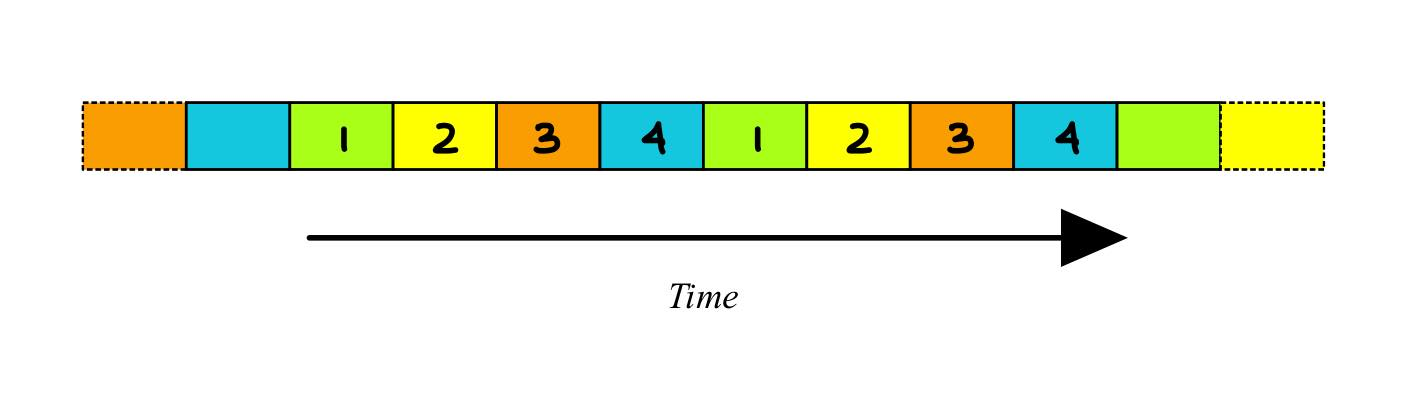
\includegraphics[width=1\textwidth]{time}
\centering
\caption{Time division multiplexing.}
\label{fig:time}
\end{figure}

Although the traditional outline employs a circular, equal-time division, it is possible to assign priority in terms of statistical information, be it from delivery or receipt of information through the system's complete history. Under this, the protocol adopts the better name of statistical time division multiplexing (STDM).

\subsection{Multithreading}

A process thread is a unit of processor utilization that permits the running of a set of operations within the core of the computer. Modern computers permit the capability of running multiple threads in a single processor. This allows the event of running various processes simultaneously.

While this seems to propose the opportunity to run processes in parallel, it does not work like that. Threads are concurrent: they each advance step by step waiting for the others to continue. Because they interrupt each other little by little at the high frequencies of the computer clock, it can be felt that they operate asynchronously.

The act of running different threads in a single core to apparent a parallel process is called multithreading. Because they do not work in parallel, frequently problems arise relating to the synchronization of resources, where threads may quarrel between each other of the utilization of one. Another problem can be if the threads wait each other to finish, creating a cycle that will never end. This event is termed a deadlock in computer science.

\subsubsection{Dining Philosophers Problem}

To solve the problem, a mind experiment was performed by computer scientists Edsger W. Dijkstra and Tony Hoare back in the 1960s. Let there be \emph{n} philosophers seated in a round table. Before them come plates of noodles, each for each philosopher \cite{osbook}. Fig. \ref{fig:phil} exemplifies this.

\begin{figure}[ht]
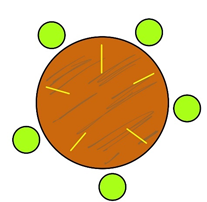
\includegraphics{phil}
\centering
\caption{Dining philosophers table.}
\label{fig:phil}
\end{figure}

To eat their noodles, they must use a pair of chopsticks. Nonetheless, they find a problem: everyone must share at least one chopstick with their adjacent neighbor. Therefore, one’s right neighbor shares their left chopstick, and the parallel with the left neighbor. Because one must use the whole pair to be able to eat, there comes the question: who eats?

The solution is very simple, although it sounds complex to implement whoever reaches the chopsticks first gets to eat first. All others who did not reach them must wait for the others to eat, hoping not to starve while waiting. When those who are eating finish, they leave the chopsticks back in the table, and let others (whoever reaches them first) to eat. To implement it in code, one must use a concept called a mutex.

A mutex is an abstract object that can be blocked so that if other threads attempt to grab them, they are unable and must wait for the process to release the mutex. Hence, they permit the synchronization of concurrent processes without the fear of robbing the resources at an inappropriate moment.

The operation to collect the mutexes if available is called \emph{wait}, because one waits for them to be free. To release them, one simply \emph{signals} the computer that they are free once again. The algorithm, short and easy, is shown below.

\begin{algorithm}[H]
\SetAlgoLined
\While{True}{
\textbf{wait} chopstick[\textit{i}]\;
\textbf{wait} chopstick[(\textit{i}+1) \% \textit{n}]\;
... \hfill\\
/* eating */\\
... \hfill\\
\textbf{signal} chopstick[\textit{i}]\;
\textbf{signal} chopstick[(\textit{i}+1) \% \textit{n}]\;
... \hfill\\
/* thinking */\\
... \hfill\\
}
\caption{Dining philosophers problem}
\end{algorithm}

\section{Experiment}

\subsection{Cases Description}

The objective of the experiments focuses on the collection of solid information for statistical comparison among the results of the crops status according to the various selected algorithms planted before. In this report, what will be displayed are computer simulations defined from the mathematical models stated in Section 2. This will save time and other resources that can be used for practical experiments on field later on.

In total, there will be four main cases. The first case (Case A) encompasses the perfect case—the scenario where there is water is fully available the whole time, and as such, the irrigation areas are kept under the best care. Every time that the humidity levels fall under the lower control threshold, the area will be watered. When it reaches the higher control threshold, it will stop to avoid waterlogging.

Case B is a bit different, as it will focus on the traditional scheme of round-robin irrigation as in time division multiplexing, following a circular pattern for the irrigation. The plants will be watered when it is established that it is their turn and they are under hydric stress. When it is not their turn, they will not receive water even if they are below the control threshold.

Case C adopts a new mannerism unto what was presented for Case B. Under Case C, once again the algorithm will be that determined under TDM. Nonetheless, it will attempt to present itself in a greedy fashion. What this means is that, even if the area reaches the higher control threshold, it will keep irrigating. What this allows is the opportunity to collect additional water while it is out of its turn. 

For the cases of the TDM application, the user provides a lapse of time of 24 hours (1,140 minutes) of allowance for the individual irrigation of the areas. Unlike the previous algorithm where the allocation of resources depend on who attains it first, TDM just demands for short periods of time defined through modular arithmetic with the formula

\begin{equation}
\label{eqn:11}
0 < t \pmod{TIME \times TOTAL\:AREAS} - TIME \times i < TIME
\end{equation}

where $t$ is the current time period in minutes, $TIME$ is the total time slot (24 hours), and $TOTAL\:AREAS$ is the total number of irrigation areas at the moment.

Lastly, Case D will make use of an adaption of the dining philosophers problem. Establishing the water tank as the equivalent of the abstract mutex object, the program will instinctively give the opportunity to the areas to irrigate if and only if no other area is being watered. That latter area will keep being irrigated until humidity reaches the upper thresholds. Right there, it will forsake the resource and let any other area take it. Keep in mind that there is no priority on who comes next; the first to solicit permission will be the one to get the water.

\section{Results}

\subsection{Plots}

In total, there were four sets of simulations. Those groups vary in similitude by the addition of different aspects in their behavior accordingly to the system dynamics representation and the algorithm or protocol for their control and regulation. Albeit four concurrent irrigation areas' behaviors were replicated, only one of them will be presented here for demonstrative reasons (Area 3).

The first collection is composed of the ideal scenario—the moment when the sensors and actuators of the plant work suitably as expected. Ideally, as it should, Case A is essentially perfect in that, even though resources are overly wasted, the system never exits from its operating point region and is at its best state. As shown in Fig. \ref{fig:case_a}, this is what should be attained given that the areas generate the greatest outcome.

\begin{figure}[ht]
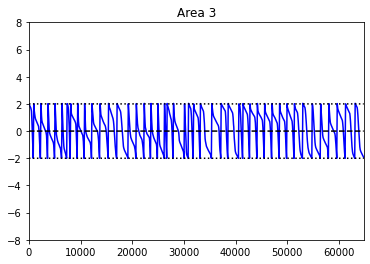
\includegraphics[width=0.5\textwidth]{case_a}
\centering
\caption{Case A - Full Water Availability.}
\label{fig:case_a}
\end{figure}

Case B presents what is expected from the conservative approaches employed routinely in agriculture nowadays.  Under TDM, because of the time-slotted division, it can be quickly inferred that it is very likely that resources will be hugely saved with this stratagem. 

Sadly, the project falls down when one understands that this comes at the price of some terrible results from the system going under constant hydric stress, signaling that it is most likely for the crop to fail in spite of the seemingly optimal use of water. This is placed in Fig. \ref{fig:case_b}. As one could observe, the irregular watering only perpetuates future damage to the vegetation.

\begin{figure}[ht]
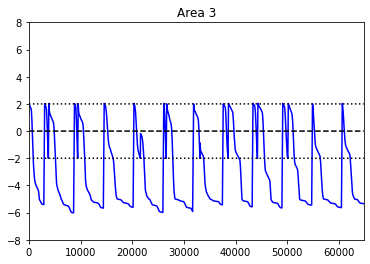
\includegraphics[width=0.5\textwidth]{case_b}
\centering
\caption{Case B - Time Division.}
\label{fig:case_b}
\end{figure}

To correct this, Case C arrives under pretense of permitting the generation of water saturation on the soil. As waterlogging occurs during the allowed turn, the areas feel safer for the moments when it is not their turn for irrigation. This greedy variation seeks to reduce any plausible and awaited risk when the area is waiting for its chance to be watered. 

While the technique indeed improves the situation, the results are not as drastic considering that more water is being wasted. Even though stress is reduced to the plant, one still not reaches the ideal scenarios from Case A. Fig. \ref{fig:case_c} introduces such images.

\begin{figure}[ht]
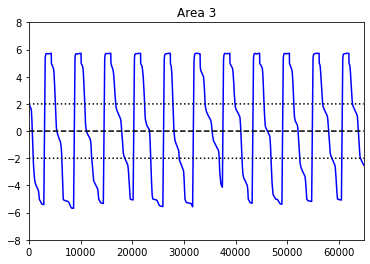
\includegraphics[width=0.5\textwidth]{case_c}
\centering
\caption{Case C - Time Division (Greedy).}
\label{fig:case_c}
\end{figure}

Now, under the dining philosophers algorithm, one will try to replicate, or at least get close, to the numeric results from Case A. This situation, known here as Case D, will include moments where the plant comes under hydric stress while it cannot irrigate, which is whenever other area is being watered and is not willing to share resources.

There are some huge notches where the plants are under some harsh hydric stress states. The reason for this is because, as water becomes utilized by any other plant, they must wait for the resource to be liberated in order to replenish. Additionally, because the areas do not follow any priority queue, it is a tournament to see who reaches first the water.

Nevertheless, what can be appreciated the most is how minor these setbacks are. The crops have an outstanding response to this strategy, given that less than 10\% percent of the time the plant is dehydrated, compared to the TDM cases. The product is displayed in Fig. \ref{fig:case_d}.

\begin{figure}[ht]
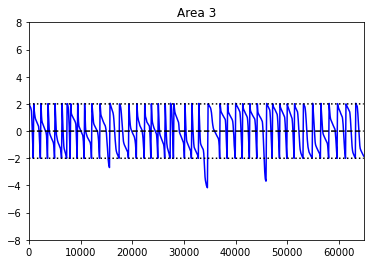
\includegraphics[width=0.5\textwidth]{case_d}
\centering
\caption{Case D - Dining Philosopher.}
\label{fig:case_d}
\end{figure}

\subsection{Numerical Data}

With the information presented before, one can compile relevant data that helps to summarize the advantages and disadvantages of all the irrigation techniques according to numerical information. What matters the most for this experiment was the total water consumption in cubic meters ($m^3$) and the percentage of time when the plant is under hydric stress (\%). The data was summarized in Table \ref{tab:results} below.

\begin{table}[ht]
\centering

\begin{tabular}{|c||c|c|}
\hline
Irrigation Technique & Water Consumption ($m^3$) & Time Stressed (\%)\\
\hline \hline
Case A & 152.145 & 0.0679 \\
\hline
Case B & 87.850 & 63.3735 \\
\hline
Case C & 554.4 & 36.1049 \\
\hline
Case D & 152.215 & 2.1898 \\
\hline
\end{tabular}

\caption{Simulation Results.}
\label{tab:results}
\end{table}

It is very evident from the start that Case A presents what is thought as the best of both worlds: an optimal consumption of water and minimal time of stress for the irrigation areas. When TDM is used in Case B, the project has a 42.26\% improvement of resource allocation taking the water into account. Unfortunately, the area is heavily put under dehydration, reaching states of 63.38\% time of water deprivation. 

This was the very reason for the modification of TDM with a greedy perspective of water collection for states of risk. While this surely reduced the period of stress to almost a half of Case B, Case D nonetheless creates an instance where water is overused and such expenses generate an unnecessary waste of the primary item in use, over four times the ideal goal of Case A.

To the moment, the alternatives based on time division have been disappointing. Case D resolves this. Ignoring the momentary instances of water deprivation, the time of stress for the plant is minimal, staying below 5\%. Additionally, water consumption is practically the same as in Case D. Their variance is essentially none.

The experiment thus shows the fantastic opportunities that can be achieved in the agricultural sector thanks to already present algorithms found in operating system theory. This algorithmic reduction implies the existence of even more techniques from computer science that can defy the conventional methods engineers tend to use in agronomy. 

\section{Conclusions}

What the experiment helped demonstrate is that these computer science concepts can be employed in any other area, and one must seize these algorithms to create an opportunity of optimization and synchronization in the daily aspects of the industrial life. Notwithstanding, this gives no right or direct pass to deploy the techniques without understanding the risks and advantages of those.

It is extremely important that, as in asymptotic complexity in the analysis of algorithms, the designer must take an effort to limit the results of the worst possible scenario. If done so, it can convey positive results by ensuring that the worst case is the optimal case, and as such, the results are utterly successful.

This is why, even time division multiplexing can have terrible descents in performance, it actually has the best resource allocation from the previously presented algorithms.

To conclude, the experiment can be considered a huge success in term of adapting a simulation model for a real system that can make use of synchronization techniques of computer science for the applications of automatic control engineering.

The next step in this arduous scientific process delves into the formalization of the experiment using a real-time embedded system architecture in an actual irrigation area. This will help to solidify the validity of the algorithm and discover any other perturbance that may be affecting the plant.

\bibliographystyle{ieeetr}
\bibliography{references}

\end{document}
